\documentclass{article}
\usepackage[shortlabels]{enumitem}
\usepackage{amsmath, amssymb, graphicx, mathtools, nicefrac, verbatim}
\usepackage[letterpaper, margin = 1in]{geometry}
\usepackage{coling2016}
\usepackage{makecell}
\usepackage{adjustbox}
\graphicspath{{imgs/}}
\newcommand{\specialcell}[2][c]{%
  \begin{tabular}[#1]{@{}c@{}}#2\end{tabular}}
\usepackage{cprotect}
\title{Group 18: 312 Project | Milestone 1}
\author{Lucian Chauvin \\ 133003371 \\\And Joshua Lass \\ 531009387 \\\And Bjorn Quarfordt \\ 230003985}
\begin{document}
\maketitle
    \vspace{-1cm}
\section{Transformation Tables}
\begin{center}
\begin{adjustbox}{width=\columnwidth,center}
\begin{tabular}{|l|l|l|l|l|l|l|}
    \hline 
    Instruction & Fetch & Decode & Execute & Memory & Write Back & PC Update	 \\
    \hline 
    \verb+rrmovq rA, rB+ & \begin{tabular}[x]{@{}l@{}}\verb+icode:ifun+$\leftarrow $ \verb+M_1[PC]+\\\verb+rA:rB+ $\leftarrow$ \verb!M_1[PC+1]!\\ \verb+valP+$\leftarrow $ \verb!PC+2!\end{tabular} & \begin{tabular}[x]{@{}l@{}}\verb+valA+$ \leftarrow$ \verb+R[rA]+\\\verb+valB+$\leftarrow$ \verb+R[rB]+ \end{tabular} &  &  & \verb+R[rB]+$\leftarrow $ \verb+valA+ & \verb+PC+$\leftarrow $ \verb+valP+	 \\
    \hline
    \verb+irmovq V, rB+ & \begin{tabular}[x]{@{}l@{}}\verb+icode:ifun+ $\leftarrow $ \verb+M_1[PC]+ \\ \verb+F:rB+ $\leftarrow $ \verb!M_1[PC+1]! \\ \verb+valC+ $\leftarrow $ \verb!M_8[PC+2]! \\ \verb+PC+ $\leftarrow $ \verb!PC+10!\end{tabular} &  &  &  & \verb+R[rB]+ $\leftarrow $ \verb+valC+ & \verb+PC+ $\leftarrow $  \verb+valP+	 \\
    \hline
    \verb+rmmovq rA, D(rB)+ & \begin{tabular}[x]{@{}l@{}}\verb+icode:ifun+ $\leftarrow$  \verb+M_1[PC]+\\\verb+rA:rB+ $\leftarrow$ \verb!M_1[PC+1]! \\ \verb+valC+ $\leftarrow$ \verb!M_8[PC+2]! \\ \verb!valP! $\leftarrow$ \verb!PC+10! \end{tabular}& \begin{tabular}[x]{@{}l@{}}\verb+valA+$ \leftarrow$ \verb+R[rA]+\\\verb+valB+$\leftarrow$ \verb+R[rB]+\end{tabular} & \verb+valE+$\leftarrow$\verb!valB+valC! & \verb+M_8[valE]+$\leftarrow $ \verb+valA+ &  & \verb+PC+ $\leftarrow $ \verb+valP+	 \\
    \hline
    \verb+mrmovq D(rB), rA+ & \begin{tabular}[x]{@{}l@{}}\verb+icode:ifun+ $\leftarrow$  \verb+M_1[PC]+\\\verb+rA:rB+ $\leftarrow$ \verb!M_1[PC+1]! \\ \verb+valC+ $\leftarrow$ \verb!M_8[PC+2]! \\ \verb!valP! $\leftarrow$ \verb!PC+10! \end{tabular}& \begin{tabular}[x]{@{}l@{}}\verb+valB+$\leftarrow$ \verb+R[rB]+\end{tabular} & \verb+valE+$\leftarrow$\verb!valB+valC! &\verb+valM+ $\leftarrow $ \verb+M_8[valE]+ & \verb+R[rA]+$\leftarrow $ \verb+valM+ & \verb+PC+ $\leftarrow $ \verb+valP+	 \\
    \hline
        \verb+OPq rA, rB+ & \begin{tabular}[x]{@{}l@{}}\verb+icode:ifun+$\leftarrow $ \verb+M_1[PC]+\\\verb+rA:rB+ $\leftarrow$ \verb!M_1[PC+1]!\\ \verb+valP+$\leftarrow $ \verb!PC+2!\end{tabular} & \begin{tabular}[x]{@{}l@{}}\verb+valA+$ \leftarrow$ \verb+R[rA]+\\\verb+valB+$\leftarrow$ \verb+R[rB]+ \end{tabular} & \verb+valE+$\leftarrow $ \verb+valB OP valA+ &  & \verb+R[rB]+$\leftarrow $ \verb+valE+ & \verb+PC+$\leftarrow $ \verb+valP+	 \\
        \hline
    \verb+jXX Dest+ &  &  &  &  &  & 	 \\
    \hline
    \verb+cmovXX rA, rB+ &  &  &  &  &  & 	 \\
    \hline
    \verb+call Dest+ &  &  &  &  &  & 	 \\
    \hline
    \verb+ret+ &  &  &  &  &  & 	 \\
    \hline
    \verb+pushq rA+ &  &  &  &  &  & 	 \\
    \hline
    \verb+pop rA+ &  &  &  &  &  & 	 \\
    \hline
 \end{tabular}
\end{adjustbox}
\end{center}
\section{Fetch Implementation}
Our design is basically a one-to-one implementation of what is shown on the slides. Our instruction memory module stores the program in ROM and reads $10$ bytes in from the current \verb+PC+. We then pass these $10$ bytes to our align module which | based on if we need registers or not | sets out \verb+rA+, \verb+rB+, and \verb+valC+ correctly. We determine whether we need registers based on the value of \verb+icode+. Then based on if we read in registers or if we read in a  \verb+valC+ we increment our \verb+PC+ using our PC increment module.
\subsection{Fetch}
\begin{center}
    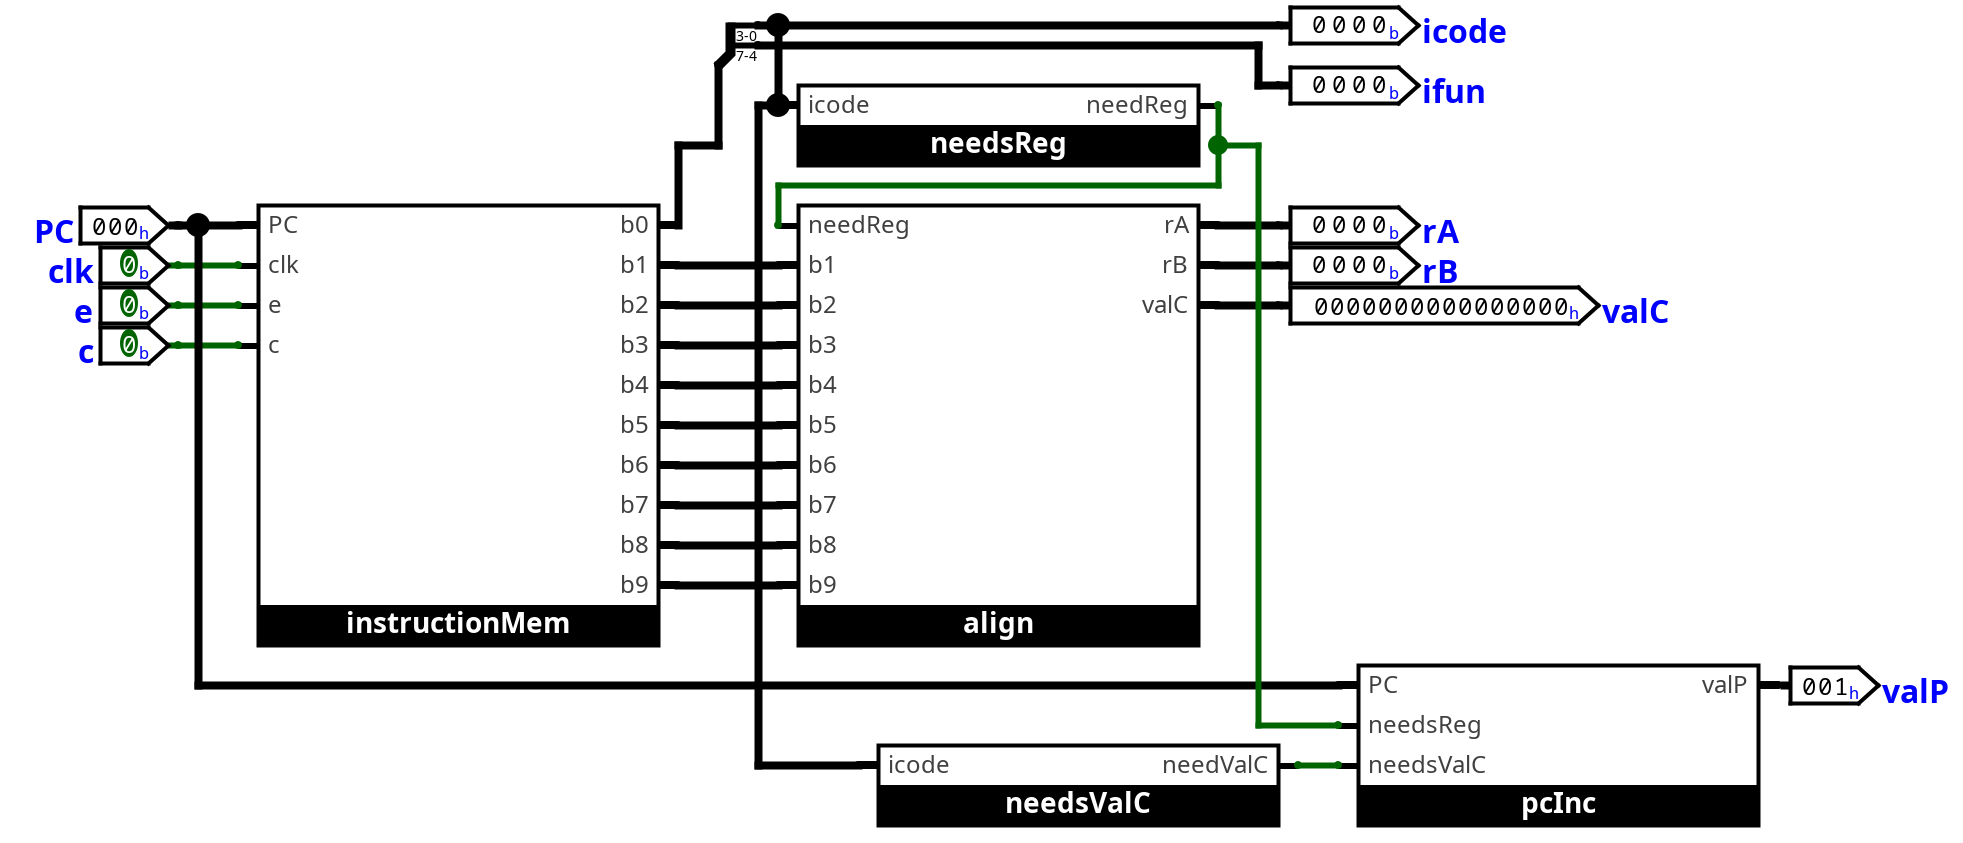
\includegraphics[scale=.7]{fetch.png}
\end{center}
\subsection{Instruction Memory}
Our instruction memory module consists of a ROM module that stores the program along with a counter and $10$ registers to store each byte of our program. Based on the counter we use a decoder to set the value of the corresponding register the count points to. We also utilize a simple 4-way \verb+AND+ gate to determine when to reset our counter. This module takes $10$ cycles to read in all $10$ bytes (one for each byte).
\begin{center}
    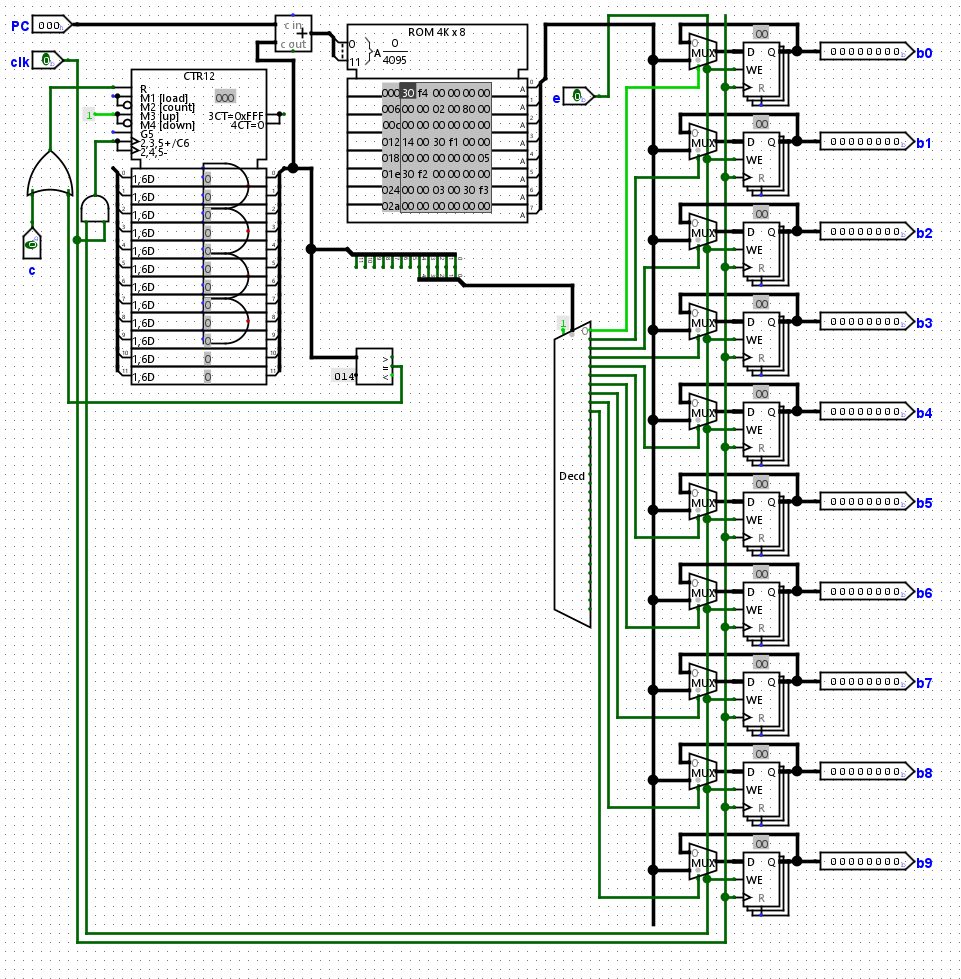
\includegraphics[scale=.45, angle=90]{instrucMem.png}
\end{center}
\subsection{Align}
The align module determines the values of \verb+rA+, \verb+rB+, and \verb+valC+ based on whether our instruction needs registers or not. When the instruction doesn't need registers we simply construct  \verb+valC+ based on the first byte being the most significant to the eighth being the least. We just let our registers still be the first byte in this case as it does not matter what is in them. When we do have registers used in our instructions we start with our most significant byte in \verb+valC+ being the second byte to the least significant being the ninth.
\begin{center}
    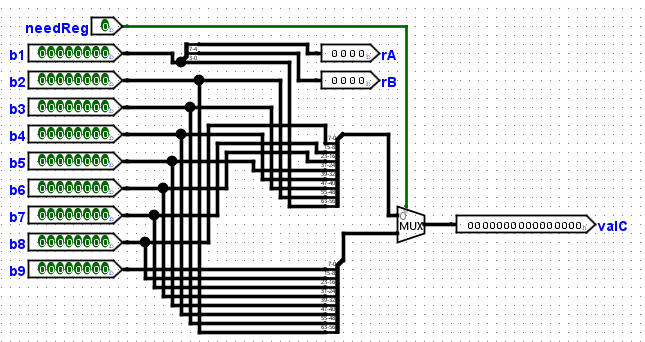
\includegraphics[scale=.7]{align.png}
\end{center}
\subsection{PC Increment}
PC increment simply increments the \verb+PC+ based on if our instruction read in registers and/or a \verb+valC+. If we read in registers we add $1$ to our \verb+PC+ and if we read in a \verb+valC+ we add $8$ to our \verb+PC+. We then also just add $1$ for our first byte containing  \verb+icode:ifun+.
\begin{center}
    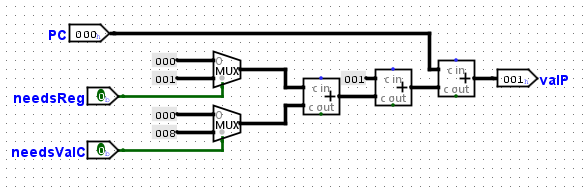
\includegraphics[scale=.5]{pcInc.png}
\end{center}
\subsection{Needs ValC and Registers}
We simply encode which instructions need a \verb+valC+ and registers based on their \verb+icode+. 
\begin{center}
    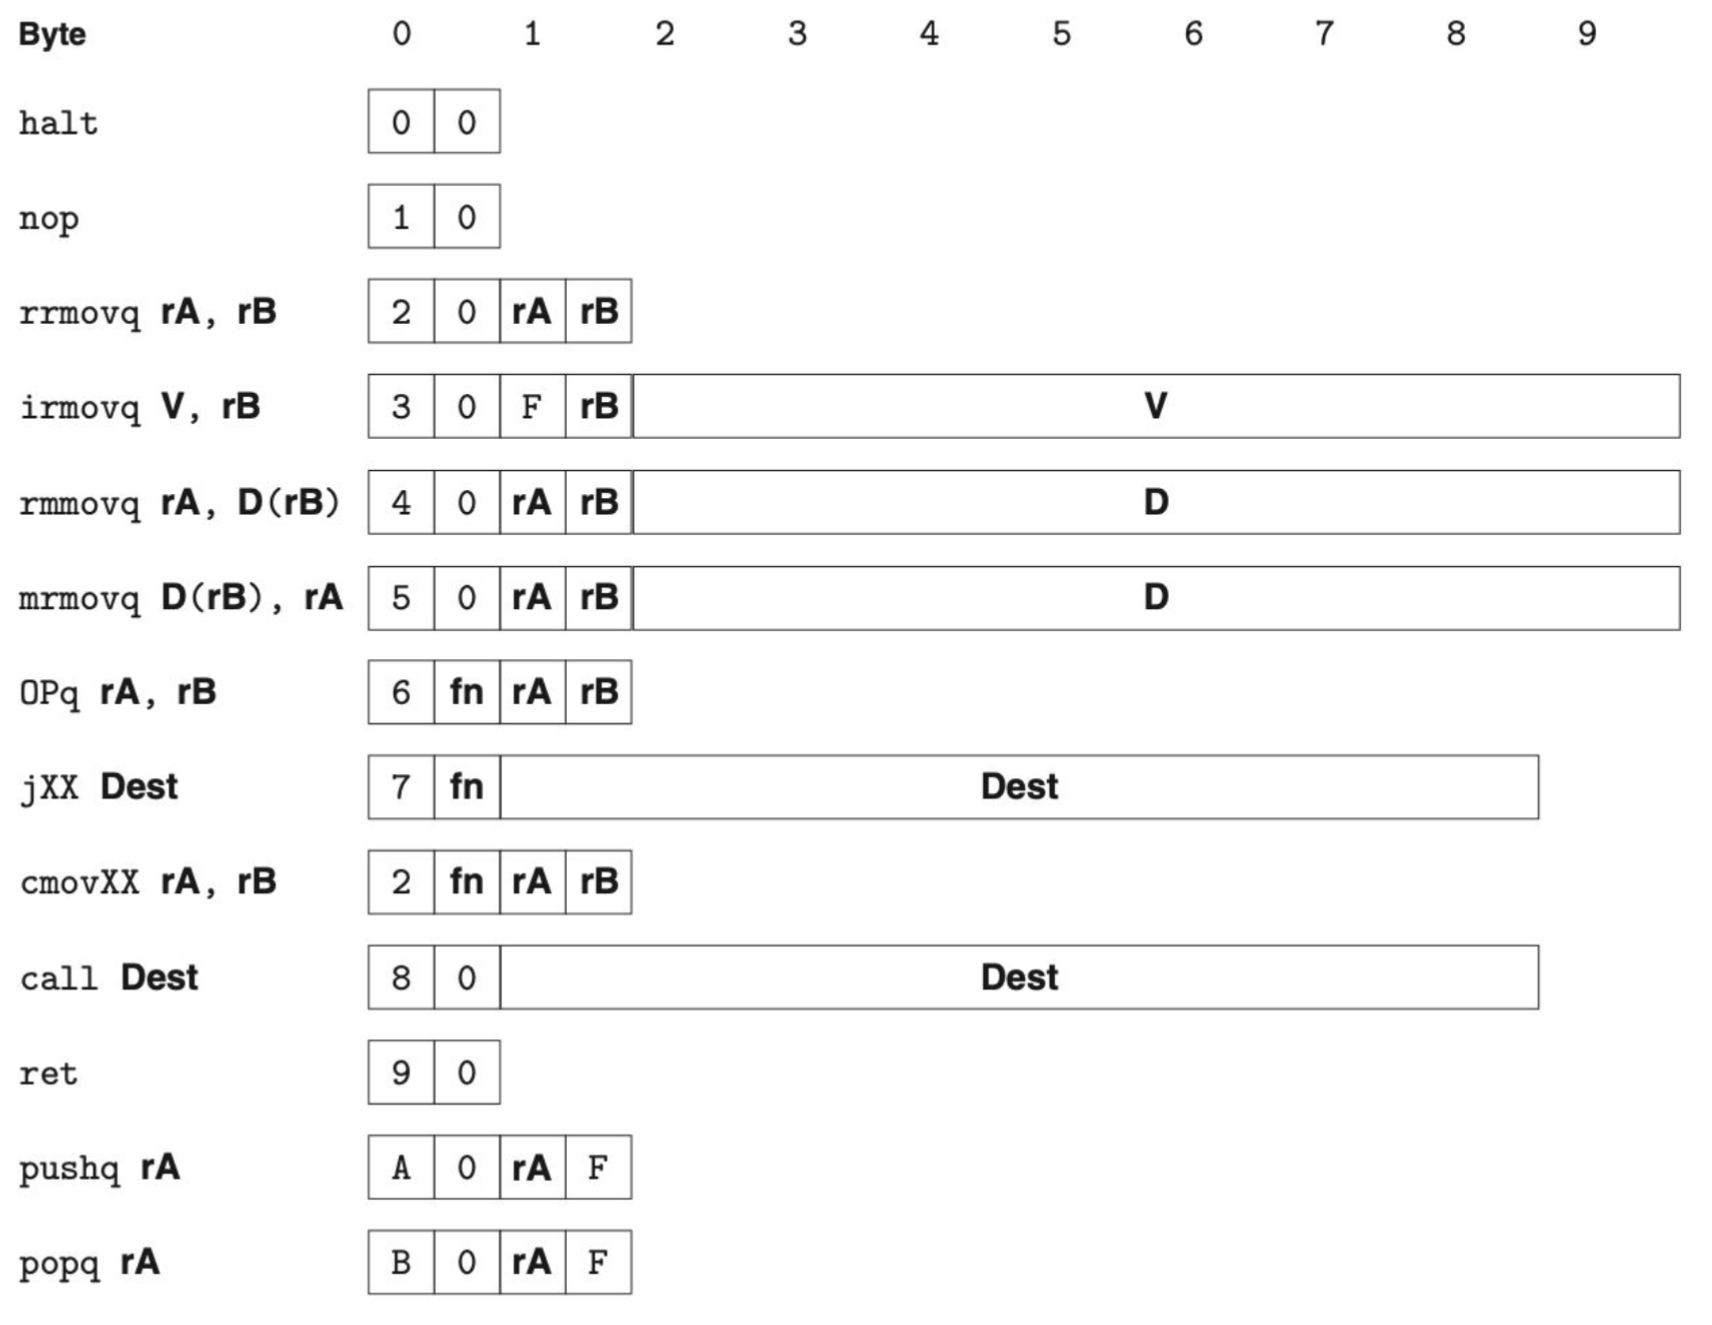
\includegraphics[scale=.6]{icode.png} \\
    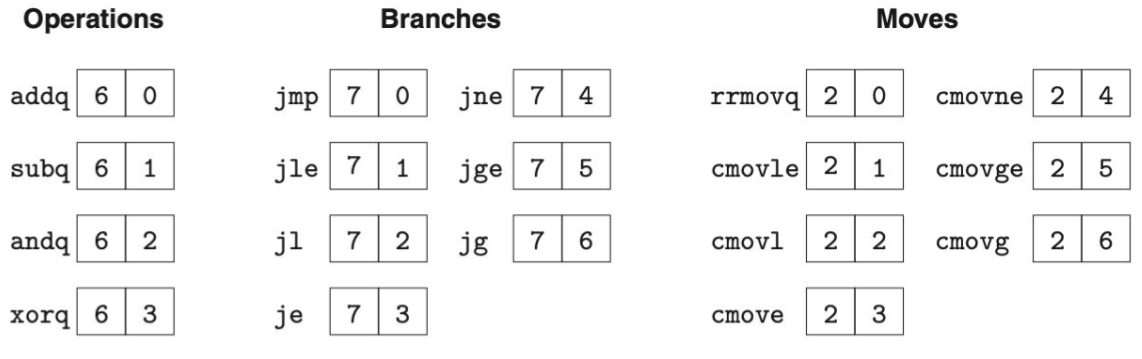
\includegraphics[scale=.8]{ops.png} 
    \\
    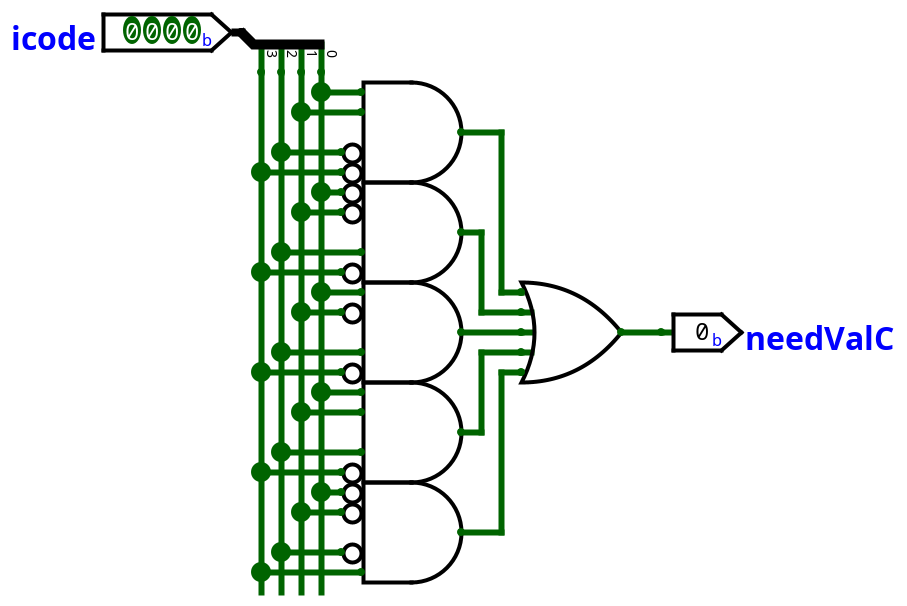
\includegraphics[scale=.7]{needsValC.png}
    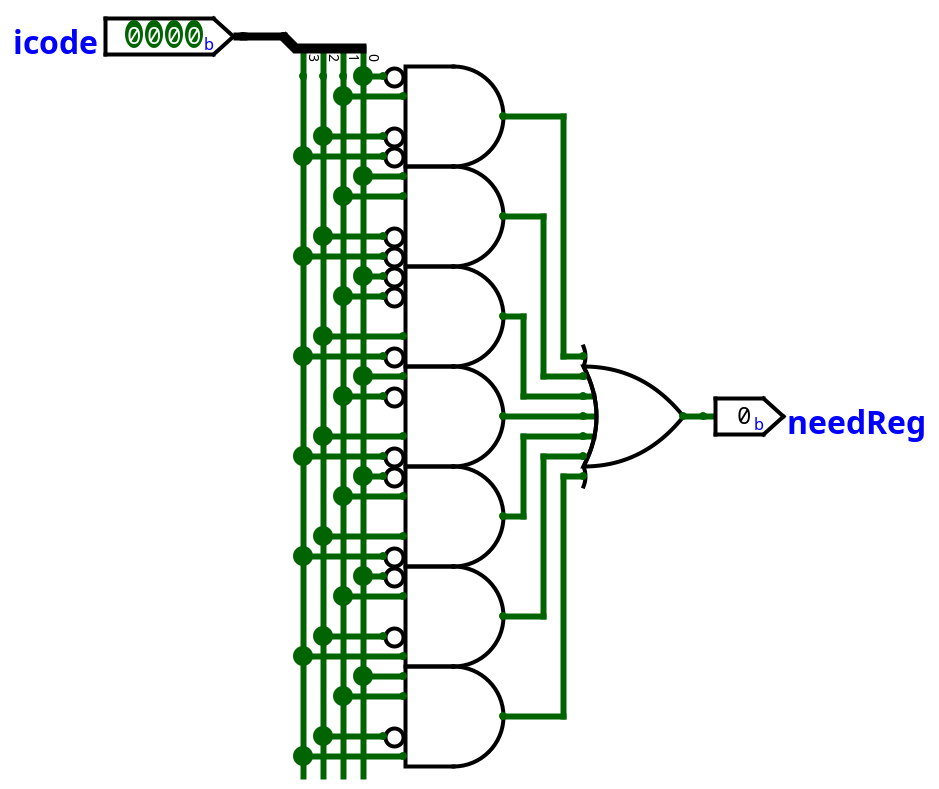
\includegraphics[scale=.7]{needsReg.png}
\end{center}
\end{document}
